\section{Image Segmentation}
The goal of Semantic Segmentation is: \\
Given an image $I$, associate to each pixel $(r,c)$ a label from $\Lambda$. \\
The result of segmentation is a map of labels containing in each pixel the estimated class.\\

Remark: segmentation does not separate different instances belonging to the same class. That would be instance segmentation. \\ \\
The training set is made of pairs $(I,GT)$, where the GT is a pixel-wise annotated imgae over the categories in $\Lambda$.

\subsection{Fully-Convolutional Networks}
CNNs are meant to process input of a fixed size. The \textit{convolutional} and \textit{subsampling} layers operate in a sliding manner over image having arbitrary size. The \textit{fully-connected} layer constrains the input to a fixed size. \\

\begin{wrapfigure}{r}{8cm}
    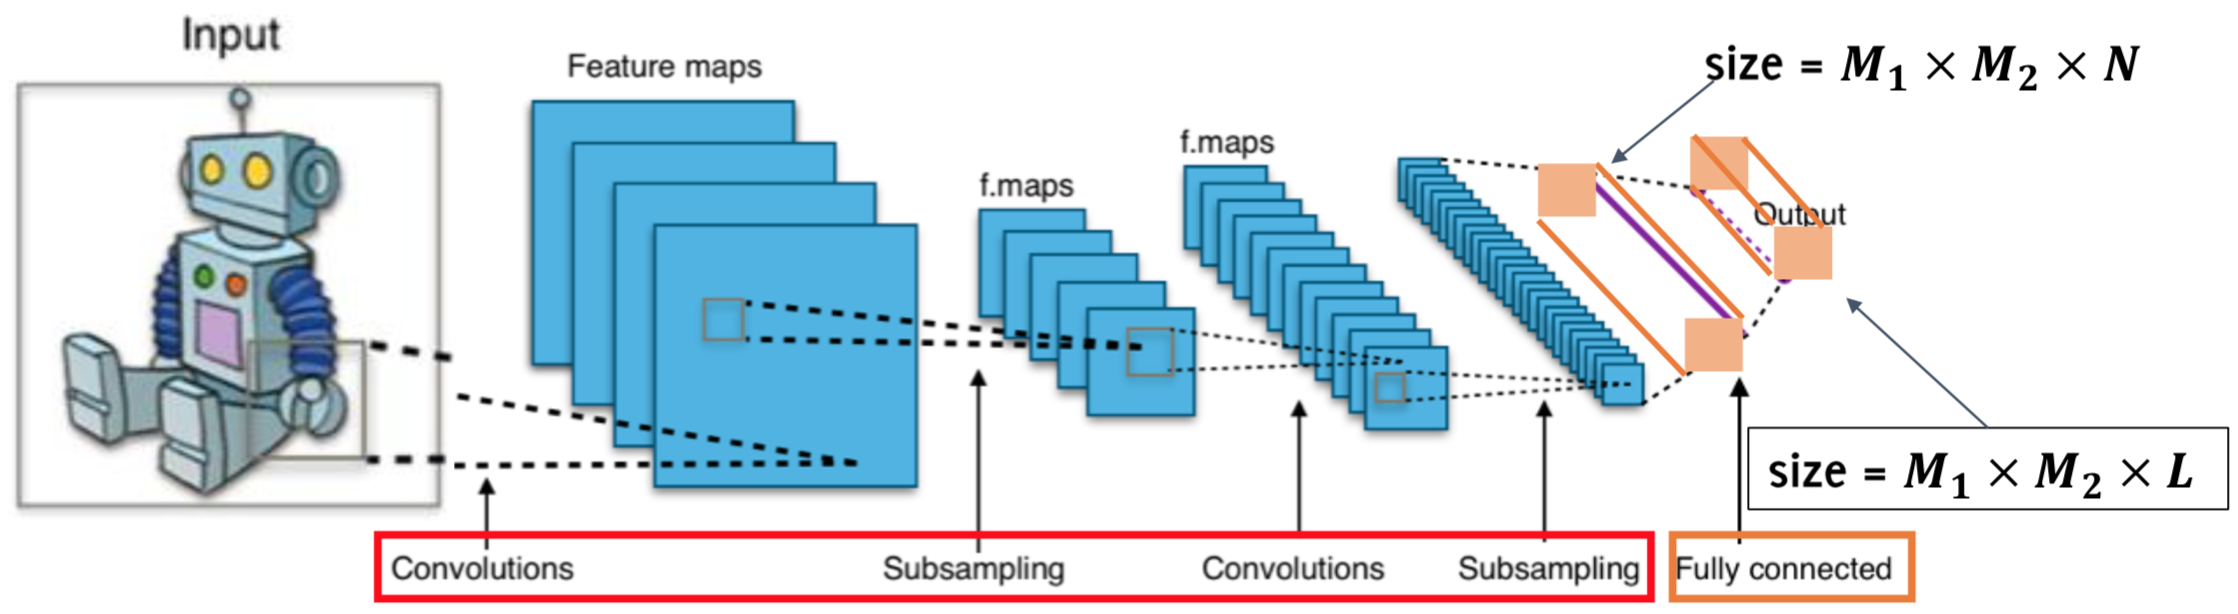
\includegraphics[width=7.5cm, height=3cm]{images/cnn_segm.png}
    %\label{fig:lstm_org}
\end{wrapfigure}  

If I fed the network with larger images, convolutional filters can be applied to volumes of any size, yielding larger volumes in the network until the FC layer. What breaks is in the FC layer because instead of having $1*1*N$, it processes a volume of size $M_1 * M_2 * N$. Thus, CNN cannot compute class scores, yet can extract features!

\begin{wrapfigure}{l}{9cm}
    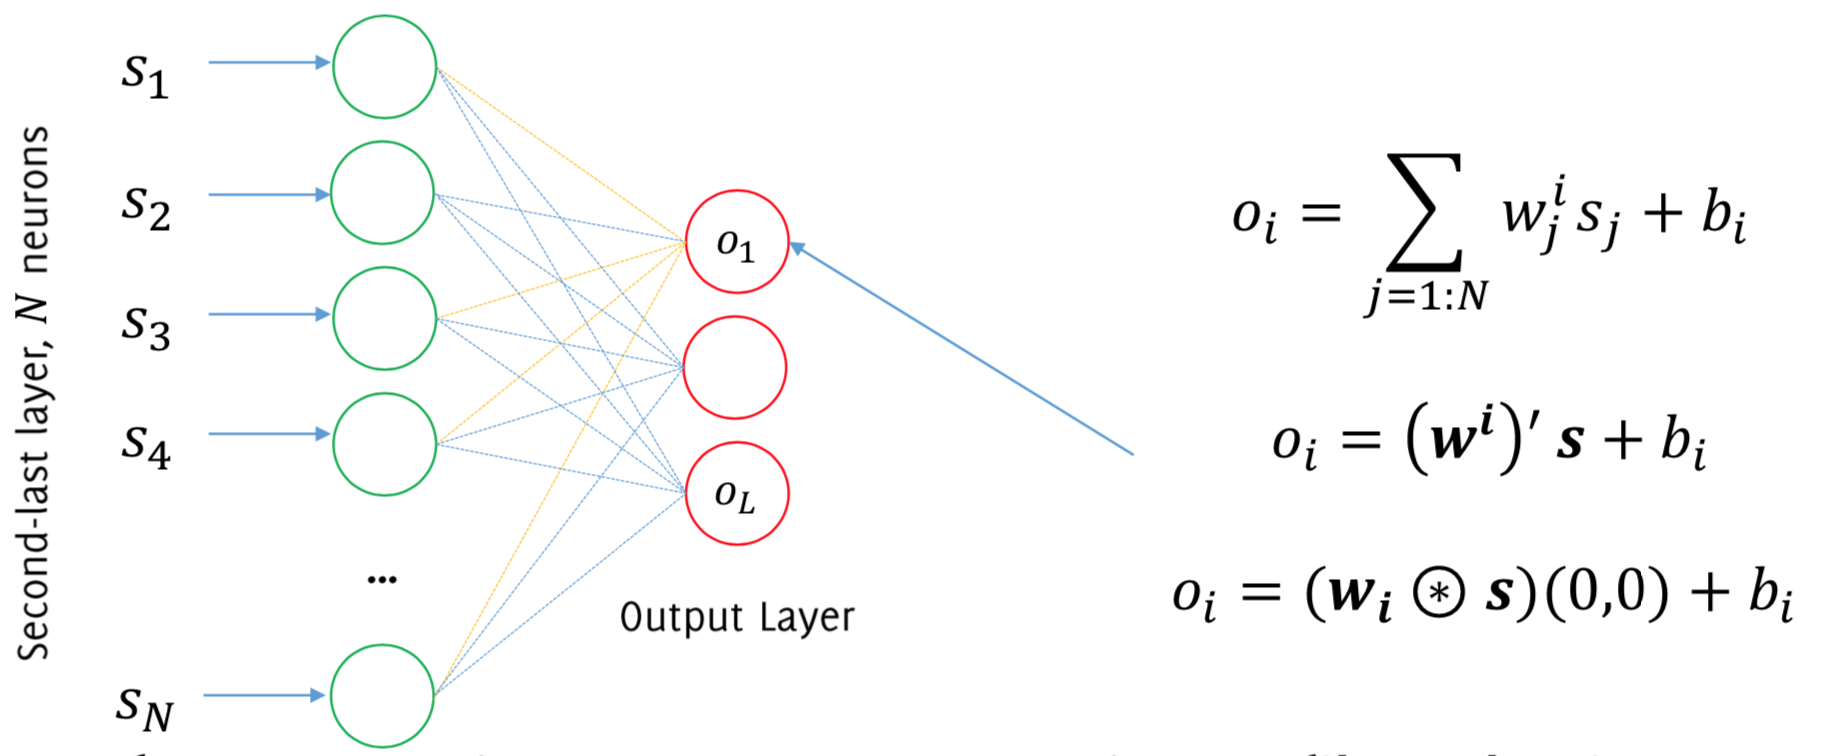
\includegraphics[width=9cm, height=3.5cm]{images/fc_to_cnn.png}
    %\label{fig:lstm_org}
\end{wrapfigure}  

However, since the \textbf{FC} is \textbf{linear}, it can be represented as convolution! Weights associated to output neuron i: $$\boldsymbol{w_i} = \left\{w_{i,j}\right\}_{i=j:N}$$ \\ \\ \\
A FC layer of $L$ outputs is a 2DConv Layer against L filters having size $1*1*N$. Each of these convolutional filters contains the weights of the FC for the corresponding output neuron. This transformation can be applied to each hidden layer of a FC network placed at the CNN top.  \\ 
For each output class we obtain an image, having: 
\begin{itemize}
    \item Lower resolution than the input image
    \item Class probabilities for the receptive field of each pixel
\end{itemize}{}

%reg.11 inizia da slide 5
%The output of segmentation can not separate between different instances (that is Instance Segmentation). 
%When we transform our model from a classification network to a Fully-Convolutional network, we can get a few heatmaps which contain for each pixel a sort of output of the scores. 
%In a cnn the first part is the entire convolutional part, then there is the fully connected one. If I change the input size of the image, the network is trained with the images of that size. If I fed the network with larger images, what breaks is in the fully connected part because instead of having a size of $1x1xN$, we obtain a size of $M_1 x M_2 x N$. You can modify a fully-connected layer which takes N input to provide L output, you can transform this (credo the fully-connected part) as a convolutional layer with convolution (qualcosa reg.12 00:44) size 1x1, and the filter has the size 1x1xN. 

%This filter has just re-writing the weights of the first output neuron.
So how many filter should I use to replace the fully-connected layer into a convolutional layer? \\
L filters: one filter per each output neuron and each filter has size $1*1*N$. We can move each fully-connected layer that takes $N$ input and provides $L$ output as a convolutional layer having $L$ filter each one having size $1*1*N$. This transformation can be applied if you have a multi-layer perceptron too.
%What the 1x1 convolution does is to mix all the filters together, all the layer together without performing any special mixing and providing this mixing as output. 
What you get is, given an image, you have multiple small images (\textit{heatmaps}), one for each classes, and these small image contains a score which tell you how much likely there is something that looks like something, for instance a wheel. 
\subsubsection{Simple Solutions}
The first way to perform segmetation is: take the heatmaps, for each pixel take the most likely class. So given an input image to fed a fully-convolutional network, you get the heatmaps: with these multiple heatmaps, for each pixel we take the argmax among those heatmaps for that pixel, which corresponds to the most probable class. However that would be a very \textbf{coarse estimate} \\

\begin{minipage}{\linewidth}
        \centering
        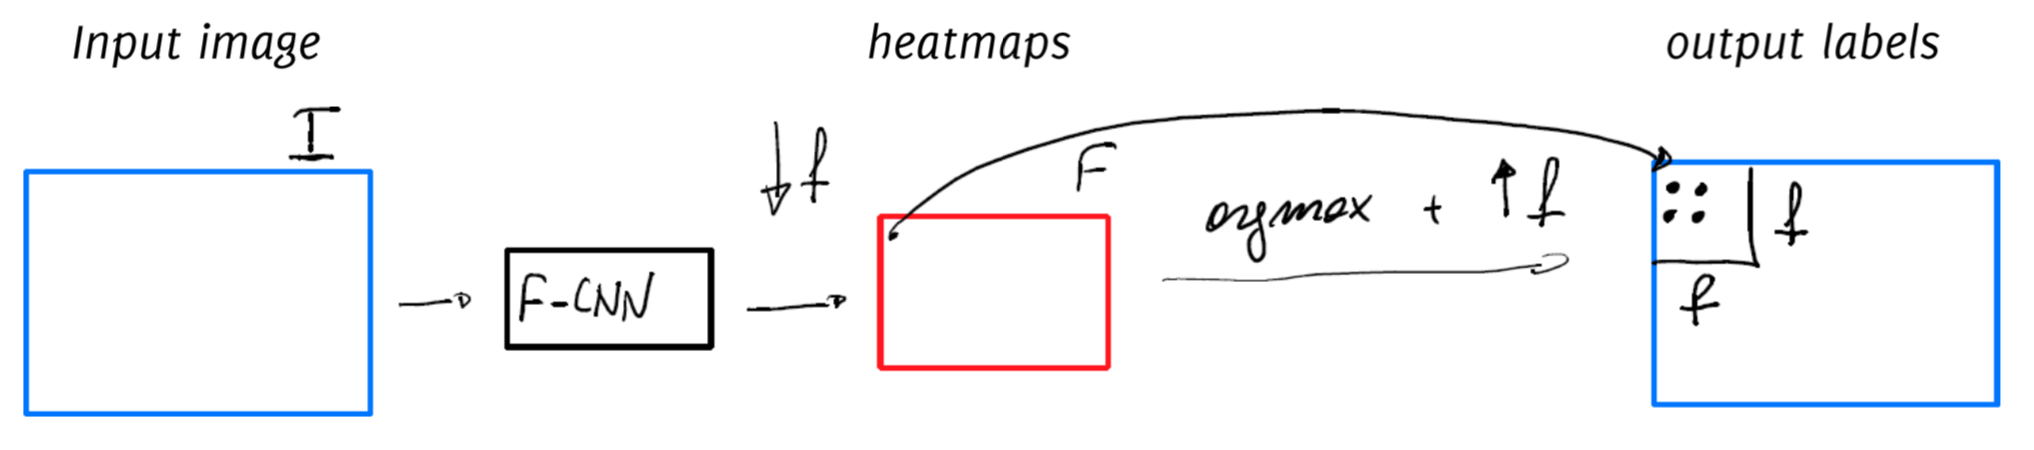
\includegraphics[width=8.1cm, height=3cm]{images/simple_solution_segm.png}
        %\captionof{figure}{The model pipeline.}
        %\label{fig:flow_fig}
\end{minipage} \\


Another option would be the \textit{Shift and Stitch}: \\
\begin{wrapfigure}{l}{9cm}
    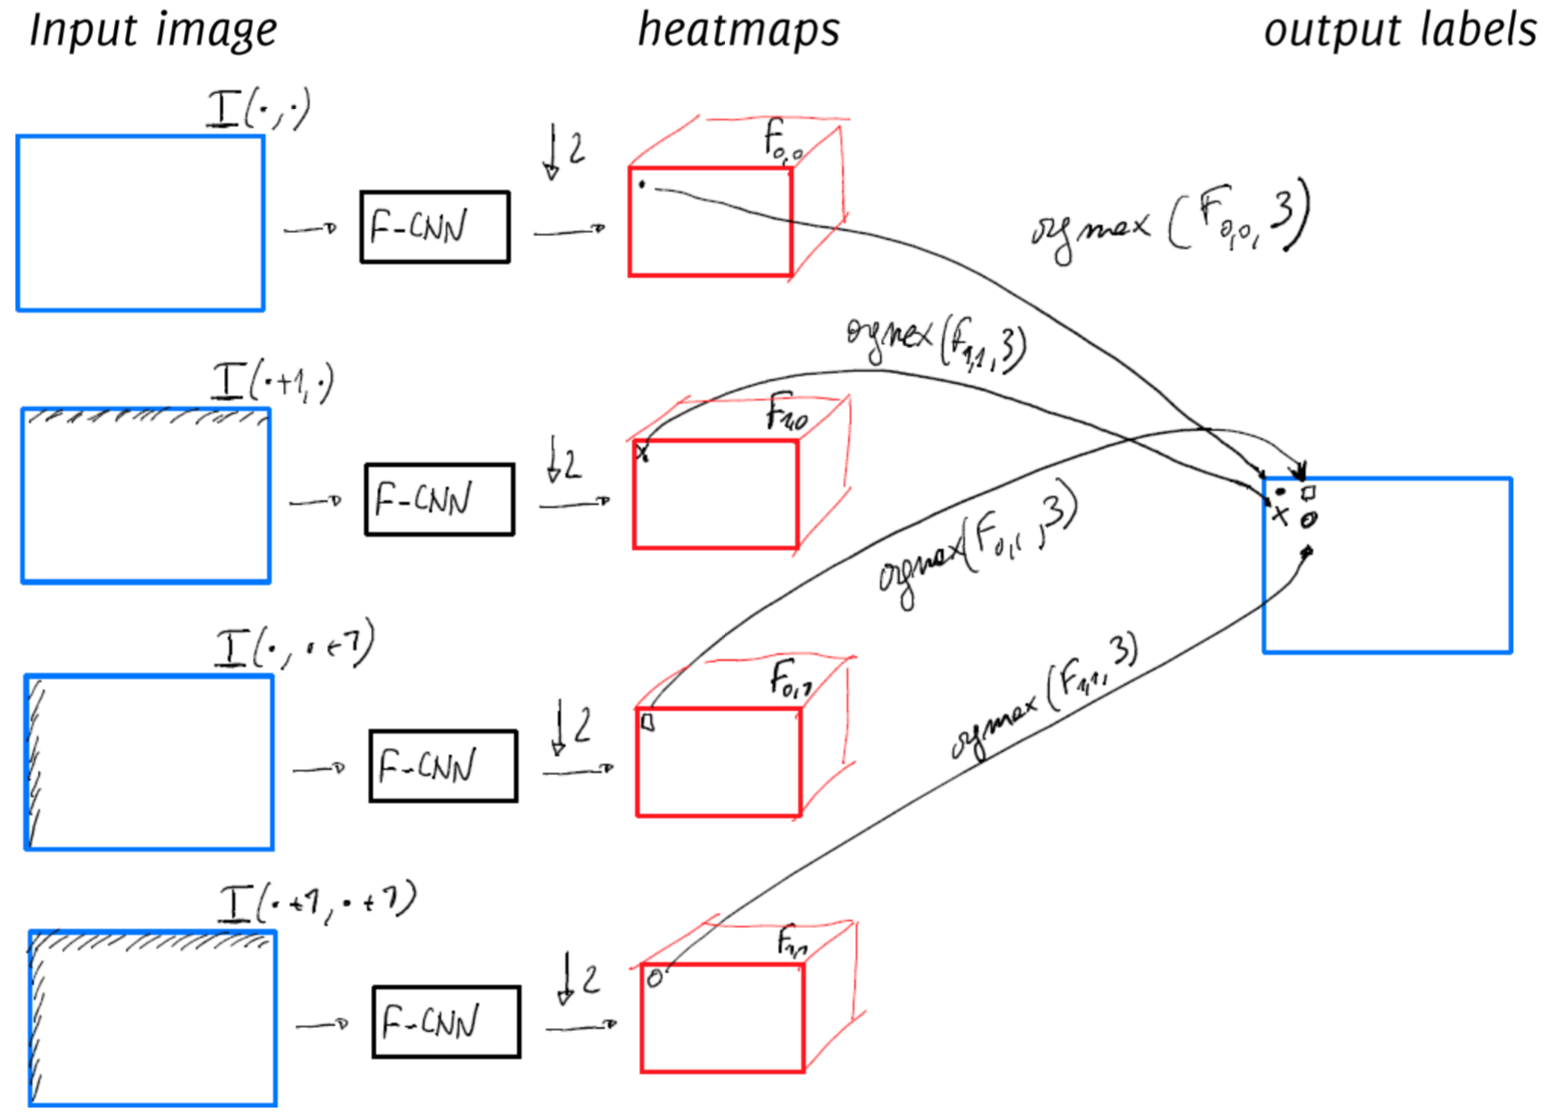
\includegraphics[width=9cm, height=8cm]{images/shift_stitch.png}
    %\label{fig:lstm_org}
\end{wrapfigure}  
Assume there is a ration $f$ between the size of the input and of the output heatmap. You have to:
\begin{itemize}
    \item Compute the heatmaps for all $f^2$ possible \textit{shifts} of the input $\left( 0\leq r, c < f \right)$
    \item Map predictions from the $f^2$ heatmaps to the image: each pixel in the heatmap provides prediction of the central pixel of the receptive field
    \item Interleave the heatmaps to form an image as large as the input
\end{itemize}{}

This exploit the whole depth of the network, however the upsampling method is very rigid. \\


%for each input image, I shift my images of 1 pixel left, 1 pixel down and so on. For each input image I make it like 4 times, with shift and without, obtaining 4 different blocks. Then there is the stich operation, given the outputs, instead of feeding only the input image, you feed also the image shifted down, the image shifted left, and the image shifted down-left. You perform the argmax and now (qualcosa incomprensibile). The major drawback of the shift and Stich operation is that is this sort of upsampling which means (this, there, there to that non si capisce una sega). \\

\begin{wrapfigure}{r}{7cm}
    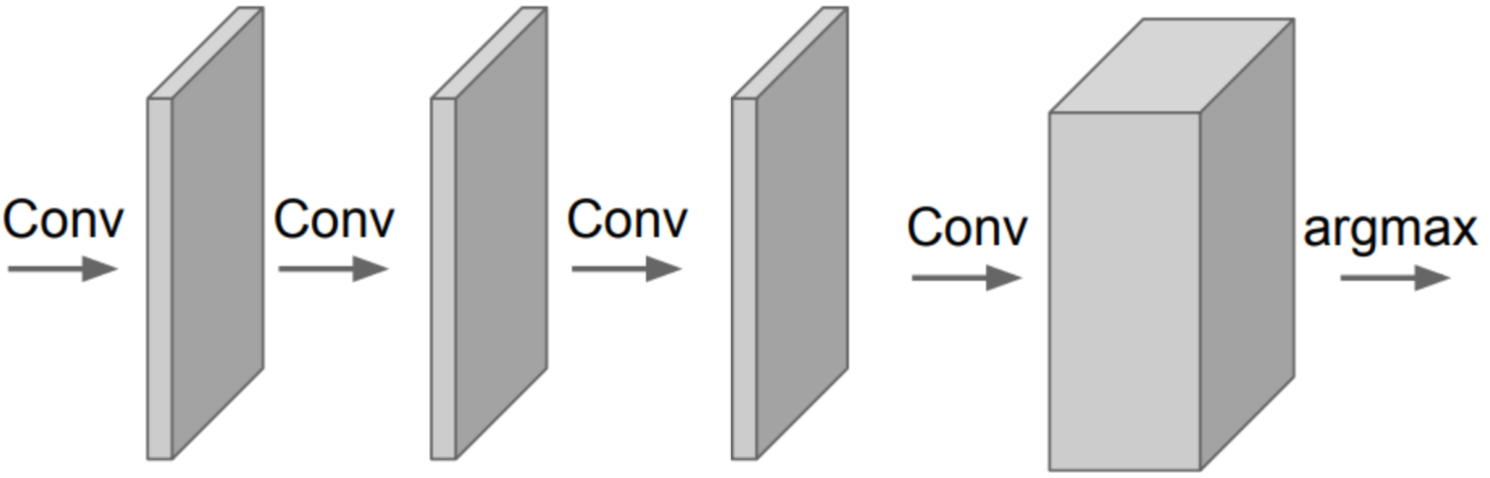
\includegraphics[width=7cm, height=3cm]{images/only_convolutions.png}
    %\label{fig:lstm_org}
\end{wrapfigure}  

The last possible approach is to perform \textit{Only Convolutions}: you can design a network without any downsampling, without any pooling. In principle, you can get in output an image with the same size, but the major drawback is that you do not increase enough the receptive field for having meaningful information $\Rightarrow$ Very inefficient. \\

\subsubsection{Main Solution}
On the one hand we need to "go deep" to extract high level information on the image. On the other hand we want to stay local not to loose spatial resolution in the predictions.\\
Semantic segmentation faces an inherent tension between semantics and location: 
\begin{itemize}
    \item global information resolves what, while
    \item local information resolves where
\end{itemize}{}
Combining fine layers and coarse layers lets the model make local predictions that respect global structure. \\
An architecture like the following would probably be more suitable for semantic segmentation: \\

\begin{minipage}{\linewidth}
        \centering
        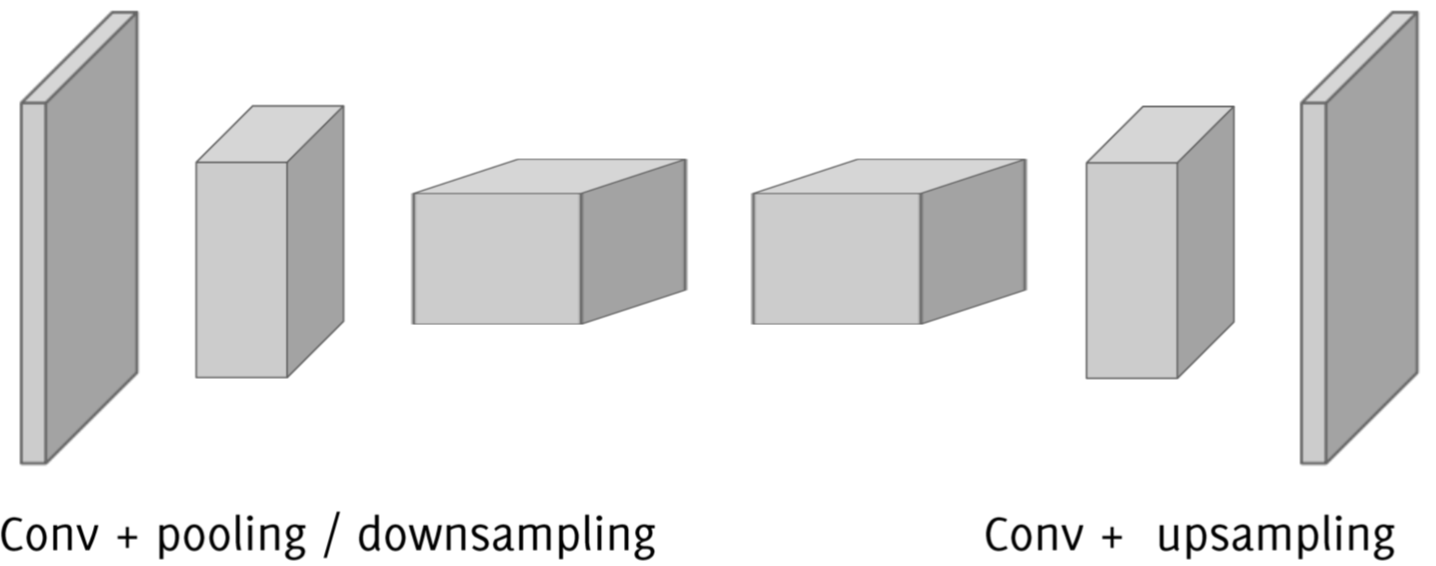
\includegraphics[width=8.1cm, height=3cm]{images/segm_architecture.png}
        %\captionof{figure}{The model pipeline.}
        %\label{fig:flow_fig}
\end{minipage} \\

In the first part you go deep encoding semantic information; in the second part, perform upsampling and get high resolution output to recover local information: this part is meant to upsample the predictions to cover each pixel in the image. Increasing the image size is necessary to obtain sharp contours and spatially detailed class predictions. 
%Another option is, if you have some problem, you can design a network without any downsampling, without any max pooling. You can get in principle in the output an image with the same size, but you do not increase enough your recepting field for having meaningful information in the final layer.
%What we want to have during segmentation is:
%'semantic segmentation faces an inherent tension between semantics and location', so in order to understand the content of the image you need to go deep, you need to have this squeezing of your volume to have some information that refers to multiple pixels. In the other have, to have accurate predictions and accurate estimate, you need to avoid this operation of squeezing and keeping the highest resolution as possible. The idea of the original paper is to combine fine layers and coarse layers to let the model make predictions over a global structure. 
%So what is said in the paper is firstly to go deep and then doing the opposite operation, so increase the spatial resolution in order to have the same input resolution. What you want is that the second half of the networks can increase the spatial resolution preserving the semantic information. 

%So we have some convolution and some upsampling. Reducing the size of these squares, you increase the size of the pixels. 
\subsection{Upsampling}
Linear upsampling of a factor $f$ can be implemented as a convolution against a filter with a fractional stride $1/f$. \\
Upsampling filters can thus be learned during network training. \\
Upsampling can be performed in several ways: 
\begin{itemize}
    \item Nearest-Neighbor: the output is of a larger size and the pixel value correspond to the value of the nearest pixel.
    \item Bed of Nails: the output pixels correspond to the input ones, located in the top left corner of the output sub-squares, and the remaining pixels are filled with zeros.
    \item \textbf{Max Unpooling}: you have to keep track of the locations of the max during max-pooling. Remember which element was the max and, during max unpooling phase, use those positions to upsample the input and locate the max valued pixel in the same position as original.
\end{itemize}{}

\begin{minipage}{\linewidth}
        \centering
        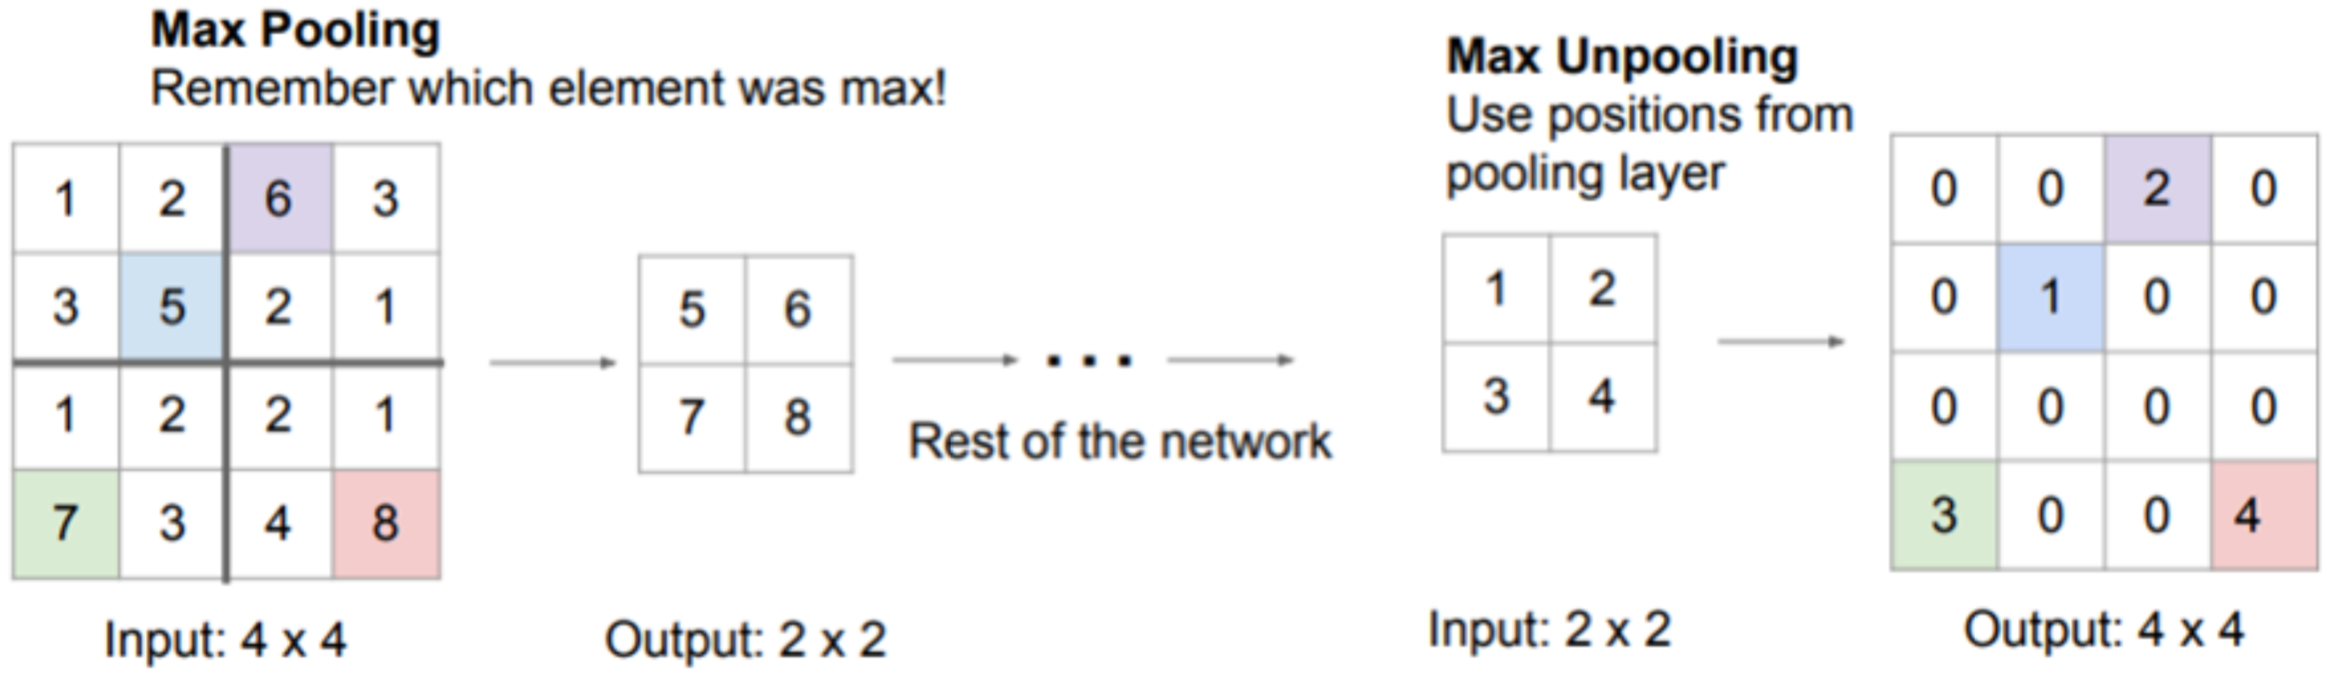
\includegraphics[width=15cm, height=5cm]{images/max_pooling.png}
        %\captionof{figure}{Logical Architecture}
        \label{fig:log_arch}
\end{minipage} \\

How to perform upsampling?\\
\textbf{Transpose Convolution} can be seen as a traditional convolution after having upsampled the input image. In this way our network can learn how to upsample optimally. \\
A classical convolution operation forms a many-to-one relationship: in general, the convolution operation calculates the sum of the element-wise multiplication between the input matrix and the kernel matrix; from a matrix you get only one value.  \\ \\
The idea of Transpose Convolution is to going backward, it's a one-to-many relationship: we want to associate one value to a matrix of values. If your input is a $2*2$ matrix, you want a $4*4$ output and you have a filter of size $3*3$ [stride 2, pad 1], get the first pixel value of the input and multiply it by the kernel values: this operation returns a filter that has been rescaled by the value of the image, so the input gives weight for the $3*3$ filter. Compute the same operation for the other pixels and sum the values where output overlaps. \\

\begin{minipage}{\linewidth}
        \centering
        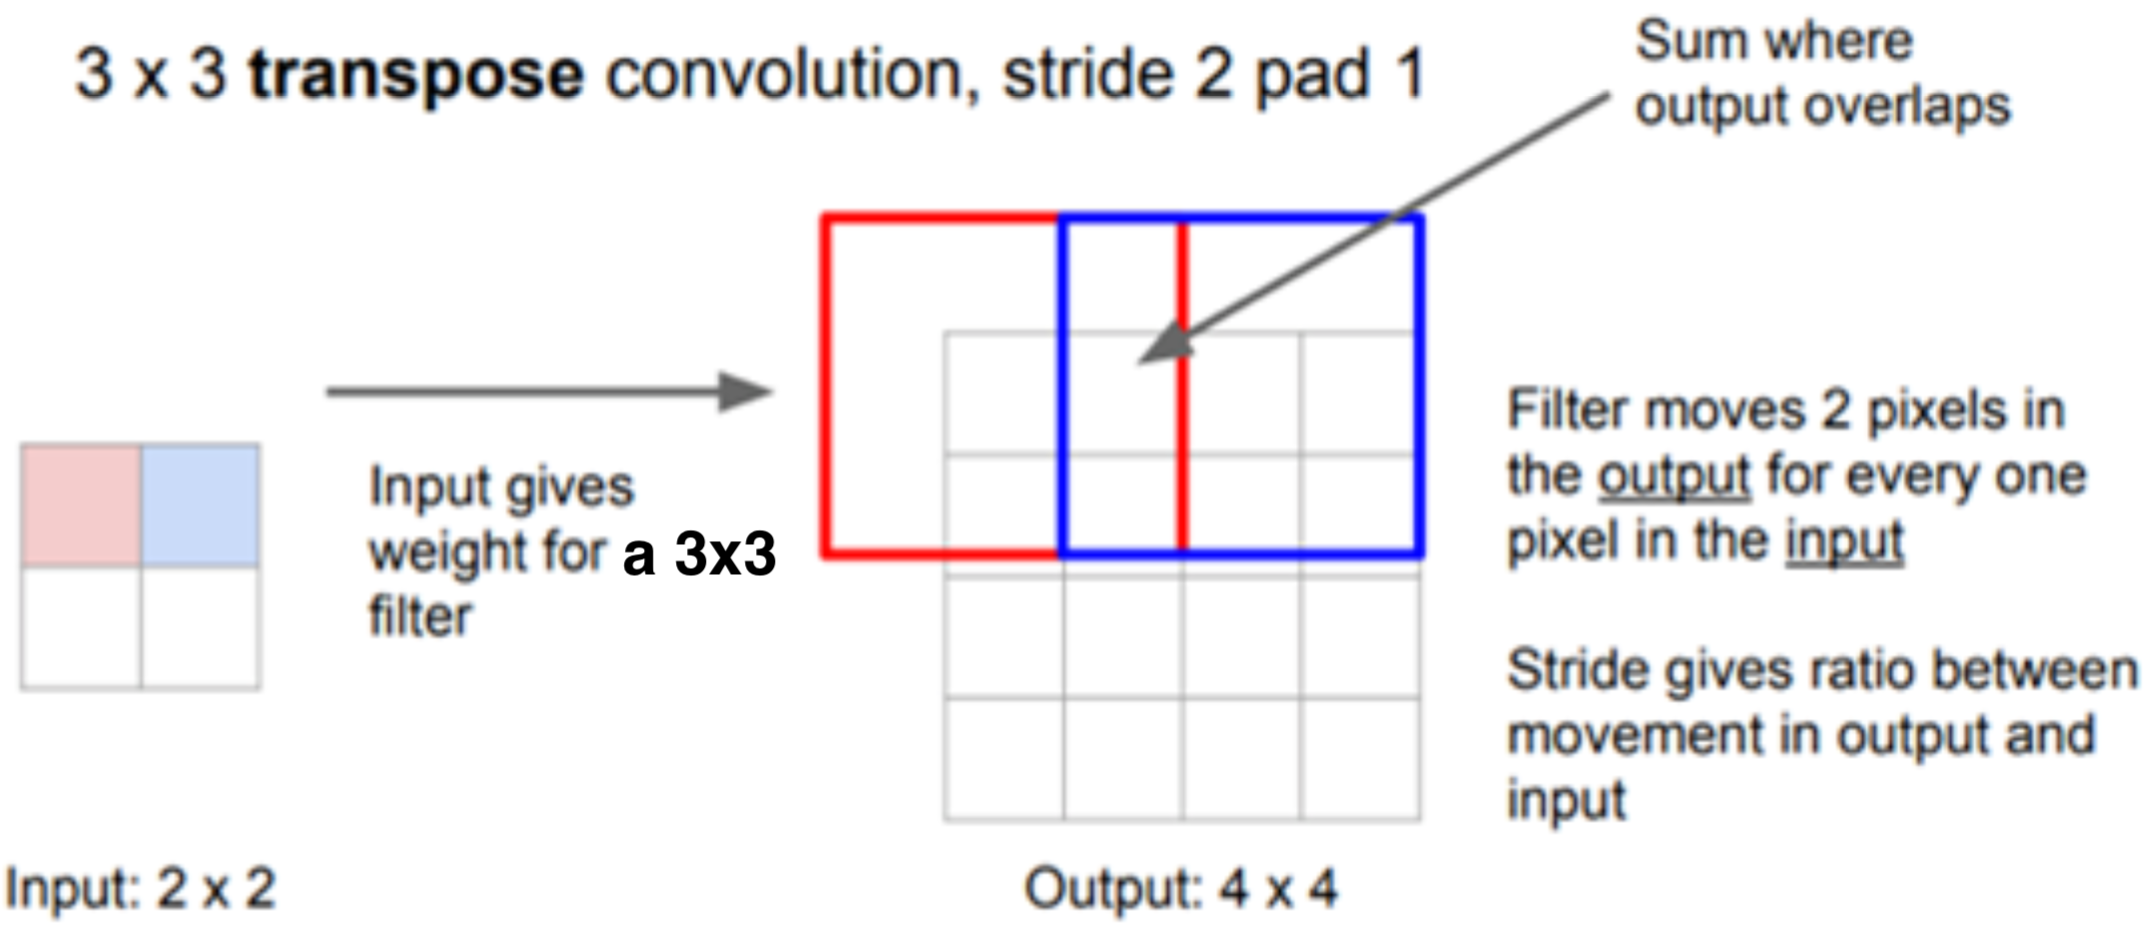
\includegraphics[width=15cm, height=5cm]{images/transpose_conv.png}
        %\captionof{figure}{Logical Architecture}
        \label{fig:log_arch}
\end{minipage} \\ 

%There are standard upsampling option like nearest-neighbours: the output is of a larger size and the pixel value correspond to the value of the nearest pixel. There is max-unpooling: when you perform the max pooling, you keep track of the location where the maximum was. So if there is the input in the contractive part of the network [so 5,6,7,8 nell'immagine] and instead of keeping the max values and propagate to the network, you keep track of the location inside the activation maps where these pixels were. So when you get back to the same point in the network to the corresponding layer you put the max values in the original location where they were. In this way you double the image size. 
%The idea of how to perform this parametric upsampling, it through the \textbf{Transpose Convolution}: change the role of the filter of the image; the input is 2x2 and you want a 4x4 output and you have a filter 3x3. So the transpose convolution is like, you take the value of the 2x2 image and you multiply it by you 3x3 filter and this gives you as output a filter that has been rescale by the value of the image. Then you place these values and you actually obtain 9 estimate, each one equal to the value of the filter rescale by the value of the image. Then you move by one pixel (depend on the filter definition) and you take this value of the image and you multiply by the same filter and you get 9 estimation. Then you sub the values on those location where the outputs overlaps. 
These predictions however are very coarse. Upsampling filters are learned with initialization equal to the bilinear interpolation. The solution is to introduce \textbf{Skip Connections}.

\subsection{Skip Connections}
There was some information that was captured in the initial layers and was required for reconstruction during the up-sampling. If we would not have used the skip architecture that information would have been lost. So the information that we had in the primary layers can be fed explicitly to the later layers using the skip architecture. \\ 

\begin{minipage}{\linewidth}
        \centering
        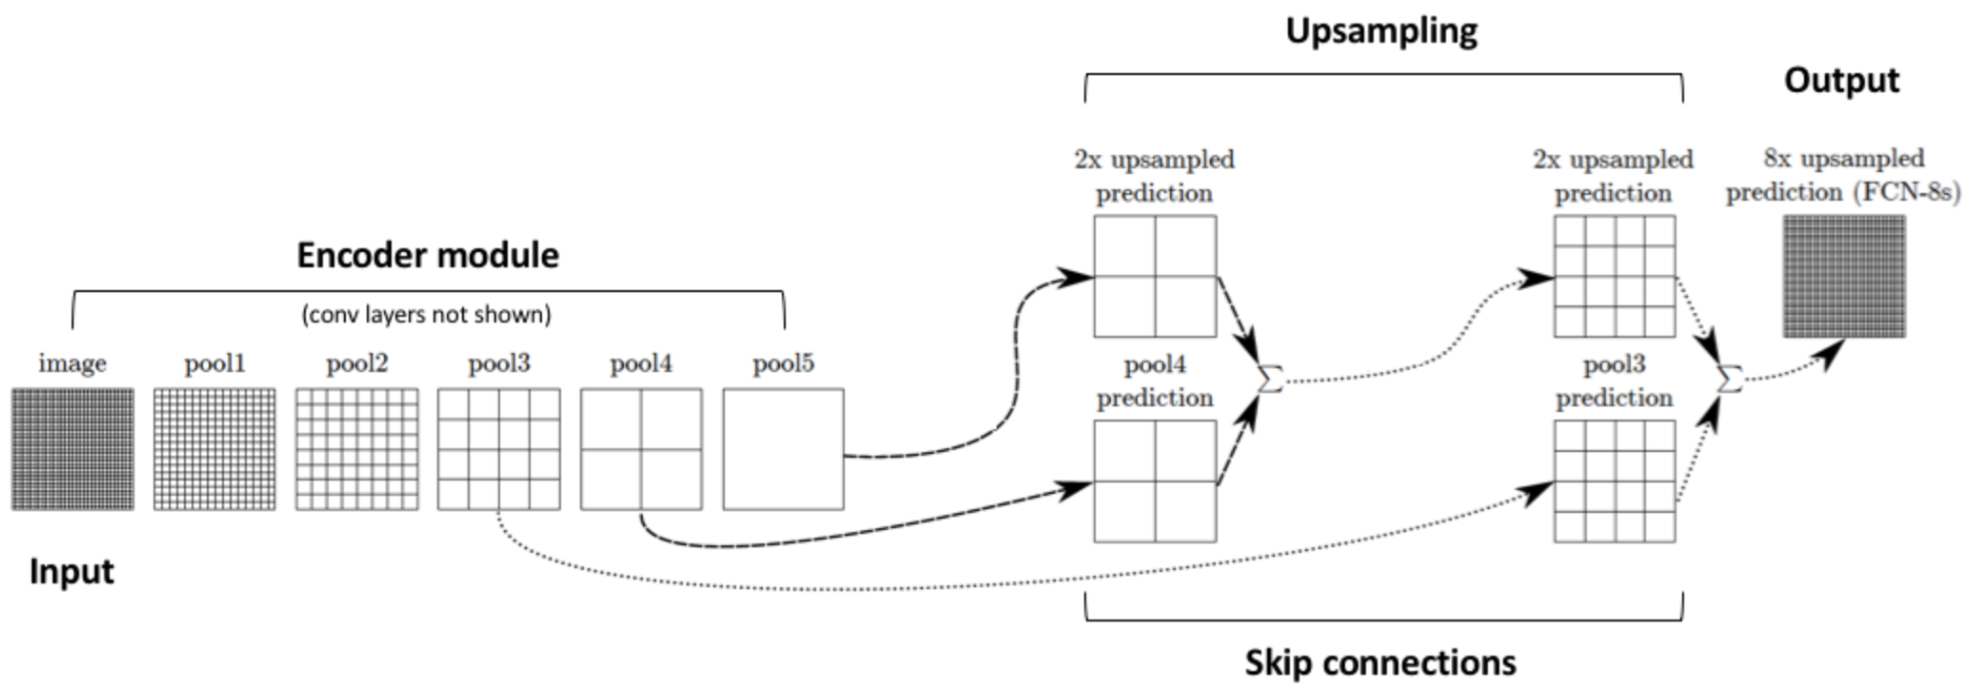
\includegraphics[width=14.5cm, height=4cm]{images/skip_connection.png}
        %\captionof{figure}{The model pipeline.}
        %\label{fig:flow_fig}
\end{minipage} \\

Supplement a traditional "contracting" network by successive layers where convolution is replaced by transpose convolution. \\
Upsampling is ubiquitous and upsampling filters are learned during training. \\
Upsampling filters are initialized using bilinear interpolation. \\
This approach yields 3 networks:
\begin{itemize}
    \item Train first the lowest resolution network (FCN-32s)
    \item Then, the weights of the next network (FCN-16s) are initialized with (FCN-32s)
    \item Tha same for FCN8s
    \item All the FC layers are converted to convolutional layers $1*1$
\end{itemize}{}

Retaining intermediate information is beneficial, the deeper layers contribute to provide a better refined estimate of segments. \\

How to train this network? \\
No need to train patchwise and then transform weights in filters. \\
It is also possible to directly train the whole network on the entire image: 
\begin{itemize}
    \item[--] Define a classification loss in each pixel
    \item[--] Average this loss over the receptive field of each pixel
\end{itemize}{}
Derivative of the sum of the losses can be easily computed and the whole network can be trained through backpropagation. \\
The \textit{patch-based} way:
\begin{enumerate}
    \item Prepare a training set for a classification network
    \item Crop as many patches $\boldsymbol{x_i}$ from annotated images and assign to each patch label corresponding to the path center
    \item Train a CNN for classification from scratches, or fine tune a pre-trained model over the segmentation classes
    \item Once trained the network, move the FC layers to $1*1$ convolutions
    \item Train the upsampling filters
\end{enumerate}{}
The classification network is trained to minimize the classification loss $l$ over a mini-batch: 
$$
\hat{\theta}=\min _{\theta} \sum_{x_{j}} \ell\left(x_{j}, \theta\right)
$$
where $\boldsymbol{x_j}$ belongs to a mini-batch. Batches of patches are randomly assembled during training. It is possible to resample patches for solving class imbalance.\\
It is very inefficient, since convolutions on overlapping patches are repeated multiple times. 

The \textit{full-image} way: 
since the network provides dense predictions, it is possible to directly train a FCNN that includes upsampling layers as well.\\
Learning becomes: 
$$
min \sum_{x_{j}} \ell\left(x_{j}, \theta\right)
$$
Where $\boldsymbol{x_j}$ are all the pixels in a region of the input image and the loss is evaluated over the corresponding labels. Therefore, each path provides already a mini-batch estimate for computing gradient.\\
The full-image way works as follows:
\begin{enumerate}
    \item FCNN are trained in an end-to-end manner
    \item No need to pass through a classification
    \item Takes advantage of FCNN efficiency, does not have to re-compute convolutional features in overlapping regions
\end{enumerate}{}

Drawbacks and solutions: 
\begin{itemize}
    \item[--] Mini-batches are assembled  randomly. Image regions are not. To make the estimated loss a bit stochastic, adopt random mask
    $$
    min\sum_{x_{j}} M\left(x_{j}\right) \ell\left(x_{j}, \theta\right)
    $$
    where $M(\boldsymbol{x_j})$ is a binary random variable
    \item[--] It is not possible to perform patch resampling to compensate for class imbalance: 
    $$
    min \sum_{x_{j}} w\left(x_{j}\right) \ell\left(x_{j}, \theta\right)
    $$
    where $w(\boldsymbol{x_j})$ is a weight that takes into account the true label $\boldsymbol{x_j}$
\end{itemize}{}

\subsubsection{Comments}
Both learning and inference can be performed on the whole-image at-a-time. Both in full-image or batch-training it is possible to perform transfer learning/fine-tuning of pre-trained classification models. \\
Accurate pixel-wise prediction is achieved by upsampling layers.\\
End-to-end training is more efficient than patch-wise training. \\
Being fully-convolutional, this network handles arbitrarily sized input.

%Skip Connection: by summing the two you can take advantage of both this special information and the semantic information that are in the very deep layer. It is the idea of the U-net. You either perform an upsamplig of factor like 32 and then you combine the upsamplig by taking the previous layer and you sum the upsampling and the previous layer.
%In practice you have three network in this way: it start with the one with coarsest resolution so the one with the upsampling of factor 32, then he initializes the factor of 16 with the same weights and all upsampling are initialized by bilinear interpolation. How do you train this sort of network? 
%What you can do is: instead of training the network with a classification loss, you are given all this annotated images with segments where each segment contains a label, you can perform a full-image training which means: given your network, and the output of the network, you can compare the estimated segmentation against the ground truth. The estimated segmentation contains for each pixel a label, the ground truth the same. The loss of your input image is the loss of all your pixels: you obtain a loss for each pixel. 

%The network works besides the image size since it is a fully-connected convolution. 

\subsection{U-Net}
It is the standard for segmentation. The network is composed by a \textit{contracting} part and an \textit{expansive} part, like an encoder-decoder architecture. \\
It takes an image as input, which goes through convolutional layers until the deepest part. Then the upsampling part of the network starts, based on skip connections to get informations of the contracting part. \\
There are no fully-connected layers: there are $L$ convolutions against filters $1*1*N$, to yield predictions out of the convolutional feature maps. \\
The output image is smaller than the input image by a constant boarder. 
Major differences w.r.t. (long et al. 2015): 
\begin{itemize}
    \item use a large number of feature channels in the upsampling part, while in (long et al. 2015) there were a few upsampling. The network become symmetric
    \item Use excessive data-augmentation by applying elastic deformations to the training images
\end{itemize}{}

\begin{wrapfigure}{l}{7cm}
    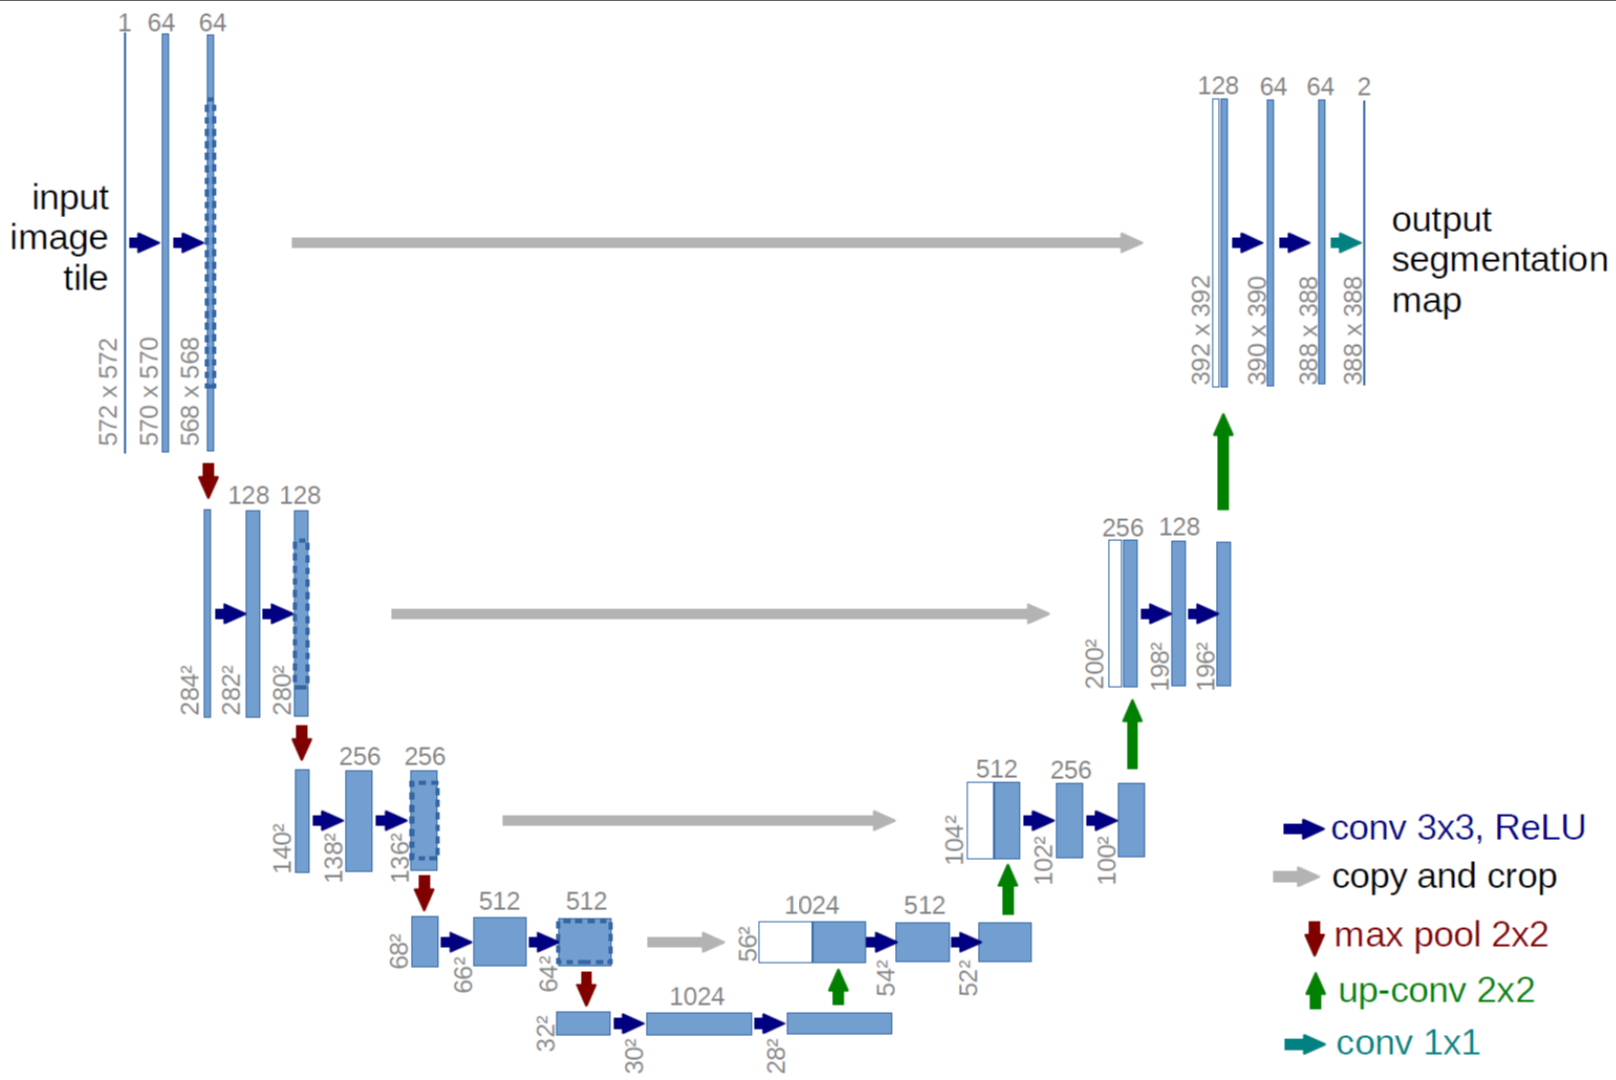
\includegraphics[width=7cm, height=5cm]{images/u_net.png}
    %\label{fig:lstm_org}
\end{wrapfigure}  

The \textit{contracting path}:\\
Repeats blocks of 
\begin{itemize}
    \item[--] $3*3$ convolution + ReLU
    \item[--] $3*3$ convolution + ReLU
    \item[--] Max-pooling $2*2$
\end{itemize}{}
At each downsampling the number of feature maps is doubled

The \textit{expanding path}:
Repeats blocks of:
\begin{itemize}
    \item[--] $2*2$ transpose convolution, halving the number of feature maps
    \item[--] Concatenation of corresponding cropped features
    \item[--] $3*3$ convolution + ReLU
    \item[--] $3*3$ convolution + ReLU
\end{itemize}{}

The main part consists in "aggregation through concatenation + convolution to mix different feature maps in a learnable manner". \\ \\
Training:\\
Full-image training by a weighted loss function:
$$
\hat{\theta}=\min _{\theta} \sum_{x_{j}} w\left(x_{j}\right) \ell\left(x_{j}, \theta\right)
$$
where the weight: 
$$
w(\boldsymbol{x})=w_{c}(\boldsymbol{x})+w_{0} e^{-\frac{\left(d_{1}(\boldsymbol{x})+d_{2}(\boldsymbol{x})\right)^{2}}{2 \sigma^{2}}}
$$
\begin{itemize}
    \item[--] $w_c$ is used to balance class proportions. $w_c(x)$ is a large number for class c that are not very representative in the training set, and it is small for class c that are very representative. 
    \item[--] $d_1$ is the distance to the boarder of the closest cell
    \item[--] $d_2$ is the distance to the boarder of the second closest cell
    \item[--] The first part of the summation takes into account class unbalance in the training set; the second part enhances classification performance at boarders of different objects: in fact, this term is large at pixels close to boarders delimiting object of different classes
    \item[--] For the second term, you have an high weight if the distance  d1 and d2 are large, where d1 and d2 are the distances between the label containing the object and the closest label that is different. Instead when d1 and d2 are small, the weights are small. 
\end{itemize}{}

%Standard for segmentation. The network is composed by a contractive part and an expansive part (encoder and decoder). It takes an image as input, which goes through convolutional layers, until it arrives to the very deepest part. Then the upsampling part of the network starts: what happens is that there are skip connections which brings the information of the contractive part of the network and what is also different is the way this information is been used: when you do upsampling, you have those 2x2 transpose convolution, but you see also that the size is increase by the depth (della parte blu) is halved, this can be done by use fewer filters (here it uses half of the filter). With the transpose convolution, you double the special extent and you copy the output from the corresponding contracting layer and you concatenate it. The upsampling part of the network is a transpose convolution concatenate with the result of the corrisponding contracting layer. In that way the network is able to recover almost the all input(?). At the end of the layer there is no fully-connected layer, it is fully-convolutional. This network is trained in a full-image map so when you measure the loss by average the predictions (forse intende averaging the error?) over the all image. In order to handle the class proportion, you weight your loss in each pixel depending on two factor: 
%\begin{itemize}
%    \item the first $w_c$: balance the class proportion. So $w_c(x)$ is a large number for class c that are not very representative in the training set, and it is small for class c that are very representative. 
%    \item the second $w_0 and so on$: it's mean to improve the classification performance at boundaries of different objects. You have an high weight if the distance  d1 and d2 are large, where d1 and d2 are the distances between the label containing the object and the closest label that is different. So when d1 and d2 are small, the weights are small. 
%\end{itemize}{}

\subsection{Global Averaging Pooling}
\subsubsection{Network in Network}
Introduce two different contributions. When you take a convolutional layer, the output is a linear combination of the inputs. So a linear combination could be too poor approximation to learn. We can use a \textbf{Mlpconv layers}: (Multi-layer-perceptron convolutional layer)
so a fully-connected network over a small portion of the input; 
instead of traditional convolutions, a stack of $1*1$ convolutions + ReLU: $1*1$ convolutions used in a stack followed by ReLU corresponds to a MLP networks used in a sliding manner on the whole image. \\
The same multi-layer perception MLP is used through all the image, this is why MLPconv layer. \\
Each layer features a more powerful functional approximation than a convolutional layer which is just linear + ReLU. \\ 

The other contribution is due to the introduction of \textbf{Global Averaging Pooling} layer: instead of a FC layer at the end of the network, compute the average of each feature map.
\begin{itemize}
    \item[--] The transformation corresponding to GAP is a block diagonal, constant matrix
    \item[--] The transformation of each layer in MLP corresponds to a dense matrix
\end{itemize}{}


\begin{wrapfigure}{r}{7cm}
    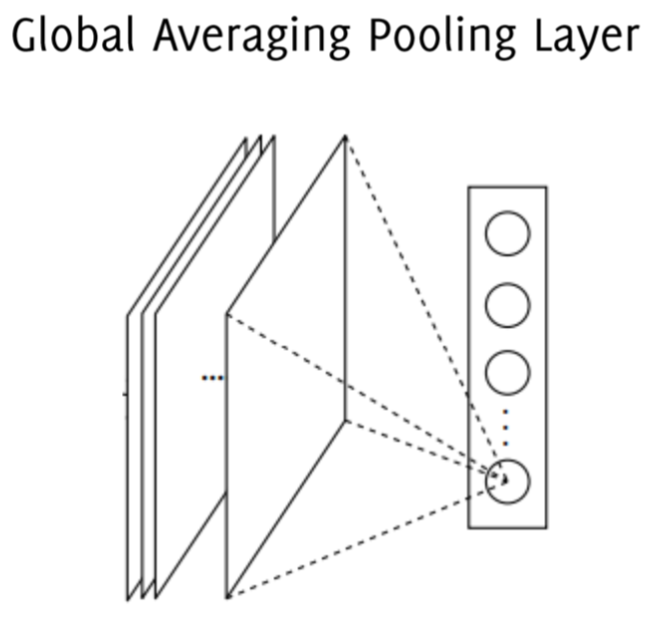
\includegraphics[width=7cm, height=5cm]{images/gap.png}
\end{wrapfigure}  

The reasons behind the introduction of GAP are that \textit{FC layers} are \textit{prone to overfitting}: they have many parameters; the dropout was proposed as a regularized that randomly sets to zero a percentage of activation in the FC layers during training. \\ \\
The GAP strategy instead is \textbf{remove the FC layer} at the end of the network and \textbf{predict by softmax} after the GAP. \\
The advantages of Global Averaging Pooling Layers:
\begin{enumerate}
    \item No parameters to optimize, lighter network less prone to overfitting
    \item More interpretability, creates a direct connection between layers and classes output
    \item This makes GAP a structural regularizer
    \item More robustness to spatial transformation of the input images
    \item The network can be used to images of different sizes
\end{enumerate}{}
Classification is performed by a softmax layer at the end of the GAP.

%Global Averaging Pooling
%Network in Network: introduce two different contribution. When you take a convolutional layer, the output is a linear combination of the inputs. So what they say is that a linear combination is too poor approximation to learn a network. What he should do is instead of having a convolution, he uses a multilayer perceptron network, so a fully-connected network over a small portion of the input and then he uses the same multi-layer perceptron through all the image. Instead of using a convolution as a filter, he uses a small multi-layer perceptron. This is called Multi-Layer Perceptron Convolutional layer (MLPconv layer) because the same multi-layer perceptron is used through all the network in a convolutional way. 

%The second point he propose is Global Averaging Pooling: it's another way to handle the fact that images may have different size; the all values over a slice here, in the deepest activation of the network, and out of all this values it simply compute the average. It takes the second slice and compute the average. At the end you have to compute the softmax over this vector of averages. If you are not interest in segmentation, what you can do when you get to the final layer of the network, you can compute the average of each layer and use the vector of the average as vector representation. 

%So the biggest advantage is that you get rid of fully-connected layer, the one with more parameter and the more prone to overfit. What was propose in the literature is to introduce dropouts between the hidden layers of the multi-layer perceptron network, as a regularizer. 

%slides 'this makes GAP a structural regualrizer': because you got less parameters and your estimate becomes less dependent on the location of a certain feature in the image, because you completely ignore the spatial extent while performing the predictions. So you have more robustness (continuare sulle slides)

